%%%%%%%%%%% CAMDA kidney data %%%%%%%%%%%%%%%
\subsection{CAMDA kidney experiment}
This is the kidney data from CAMDA (Critical Assessment 
of Microarray Data Analysis) originally described by Pritchard {\it et al}. The web-site for CAMDA is 
{\tt http://www.camda.duke.edu}. It is a 24-array double reference
design. Six samples are compared to a reference with dye swapped
and all arrays are duplicated. Flag for bad spots is included in the 
data. 

Due to the limited size of vignette, data contains only first 300 genes, and you
may not reproduce the figures presented in the following sections. You can find the original data file (in text format) at {\tt
http://www.jax.org/staff/churchill/labsite/software/}.\\ 
{\bf Read Data} Suppose you download the data and design file, then this is how you read the data. 
\begin{Sinput}
R> kidney <- read.madata(datafile="kidney.txt",designfile="kidneydesign.txt",
   arrayType='twoColor', metarow=1, metacol=2, col=3, row=4, probeid=5, intensity=7)
\end{Sinput}
{\bf Data checking and transformation} For two-color array, you need to check
if the data needs transformation. To do that you can try following data checking.  
\begin{enumerate}
\item First load data into the workspace
\begin{Sinput}
R> data(kidney)
\end{Sinput}
\item Then we do some data quality check
\begin{Sinput}
R> gridcheck(kidney.raw)
\end{Sinput}
\Rfunction{gridcheck} is used to check the hybridization 
and gridding quality within and
cross arrays. User should see near linear scatter 
plots in all grid for all arrays. 
This one is not great but acceptable. The grid check plot for the first array
is shown in Figure \ref{fig:gridcheck}. The red dots are for the spots with flags.
\begin{figure}[htbp]
\centering
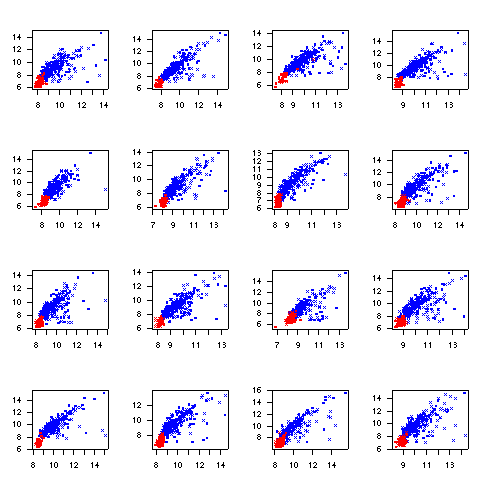
\includegraphics{gridcheck.png}
\caption{Grid check plot for the first array in kidney data}
\label{fig:gridcheck}
\end{figure}
\begin{Sinput}
R> riplot(kidney.raw)
\end{Sinput}
\Rfunction{riplot} stands for ratio-intensity plot. It is also called MA plot. 
The riplot for the first array is shown in Figure \ref{fig:riplot}. 
\begin{figure}[htbp]
\centering
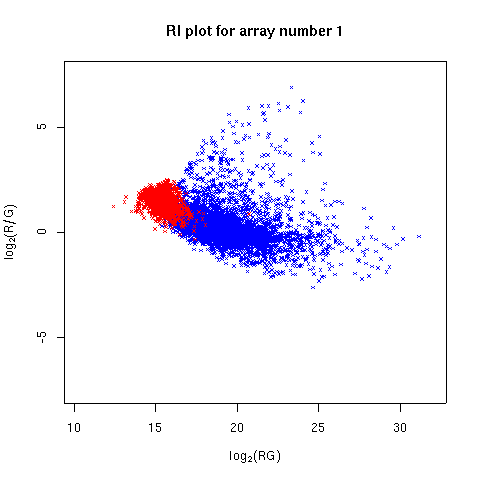
\includegraphics{riplot.png}
\caption{RI plot for the first array in kidney data}
\label{fig:riplot}
\end{figure}
\begin{Sinput}
R> arrayview(kidney.raw)
\end{Sinput}
\Rfunction{arrayview} is used to view the spatial pattern of the arrays.
The standardized log ratios for all spots are shown in different colors.
The arrayview for the first array is shown in Figure \ref{fig:arrayview}.
\begin{figure}[htbp]
\centering
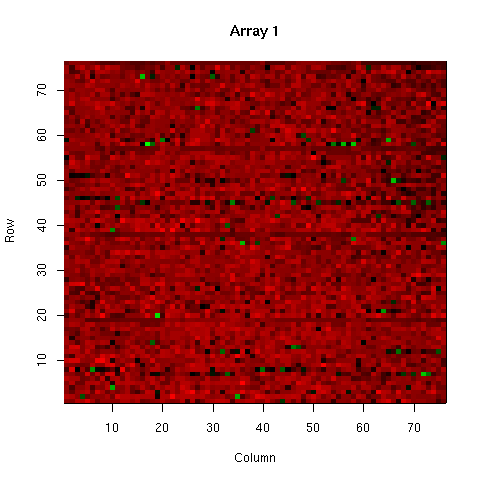
\includegraphics{arrayview.png}
\caption{Arrayview for the first array in kidney data}
\label{fig:arrayview}
\end{figure}

You will generate a lot of figures by doing 
gridcheck, riplot and arrayview. Use
\Rfunction{graphics.off()} to close all figures.
\item Transform the data using spatial-intensity joint loess.
\begin{Sinput}
R> kidney <- transform.madata(kidney.raw, method="rlowess")
\end{Sinput}
There are several data transformation method. Which method to use depends on
the data. Read Cui {\it et al.}(2002) for detail. The transformation
plot for the first array is shown in Figure \ref{fig:lowess}.
\begin{figure}[htbp]
\centering
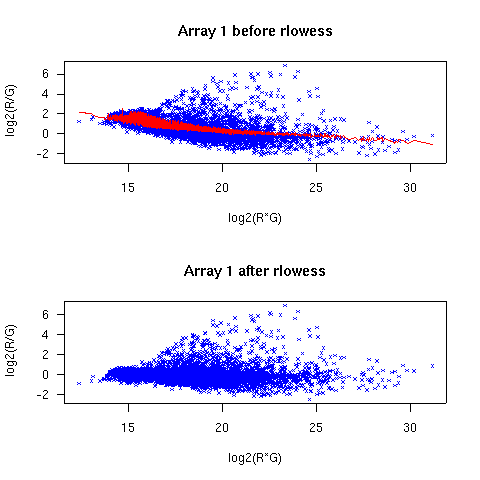
\includegraphics{rlowess.png}
\caption{Joint lowess transformation on the first array for the kidney data}
\label{fig:lowess}
\end{figure}
\end{enumerate}
{\bf Model fitting} To fit model, you need to specify \Rfunction{formula},
as well as \Rfunction{random} and \Rfunction{covariate} terms if one
has. \Rfunction{formula} includes factors affecting the gene expression among
ones specified in \Rfunction{designfile}. This also can include interactions
between upto two terms. \Rfunction{random} and \Rfunction{covariate} terms
should be included in \Rfunction{formula}. 
\Rfunction{resiplot()} shows the residual plot after model being fitted.  
\begin{Sinput}
R> fit.fix <- fitmaanova(kidney, formula = ~Dye+Array+Sample)
R> resiplot(kidney, fit.fix)
\end{Sinput}
{\bf Test statistics} To test how significantly a given term or terms affect
to the gene expression level, {\em R/maanova} calculates F, Fs and Fss test
statistics  (Fss is for fixed model only at this stage). You can include test statistics using
\Rfunction{test.method}, in which the order is F, Fs and Fss test statistics
and 1 indicates including the corresponding test statistics. As a default, {\em R/maanova} calculates F and Fs test statistics, and we recommend to use Fs test statistics.   

{\em R/maanova} provides permutation method to calculate the significance of
each test statistics. It implements residual shuffling and sample shuffling,
and sample shuffling is the current default. Permutation test could be very
time consuming, especially for the mixed effects models. The permutation
test function can run on the Linux clusters through the message passing 
interface (MPI). You need R/maanovaPR (available at {\tt
http://www.jax.org/staff/churchill/labsite/software}) package for this and for the detail information regarding F test and 
using computer cluster, please read appendix. 

Test Sample effect in the model:
\begin{Sinput}
R> test.fix <- matest(kidney, fit.fix, term="Sample", n.perm=500)
\end{Sinput}

FDR adjust p-value can be obtained using \Rfunction{adjPval}. It has four
  options;  \Rfunction{stepup} (Hochberg and Benjamini, 1990), \Rfunction{adaptive} (Benjamini and Hochberg, 2000), \Rfunction{stepdown}
  (Westfall and Young, 1993) and \Rfunction{jsFDR} (Storey,
  2002). \Rfunction{jsFDR} option uses {\em qvalue} package by John
  Storey and the package should be installed before this option
  is used. FDR adjusted P values:
\begin{Sinput}
R> test.fix <- adjPval(test.fix, method = 'jsFDR')
\end{Sinput}
{\bf Summarize the result} Each p-value or multiple testing adjusted p-value
can be found under {\tt matest()} object, i.e., p-value for Fs test statistics is
saved at \Rfunction{test.fix\$Fs\$Pvalperm} and FDR adjusted p-value for Fs
test statistics is saved at \Rfunction{test.fix\$Fs\$adjPvalperm}. \Rfunction{summarytable()} assembles
fold-change, p-value and adjusted p-value (if it is available) and the result
is saved in 'summarytable.csv' (default file name) under the working directory. User also can save subset of result using certain threshold.  
\begin{Sinput}
R> result = summarytable(kidney, test.fix)
R> summarytable(kidney, test.fix, method=c("Pvalperm"), test=c("F1", "Fs"),
whichTest=c("Fs.Pvalperm"), threshold=.1, outfile='shrotsummarytable.csv')
\end{Sinput}

After the F-test result is obtained, We can do volcano plot
to visualize it. \Rfunction{volcano()} function has options to 
choose the P-values to use and set up thresholds. We will
use tabulated P values for F and FDR adjusted permutation 
P values for other tests here. 
In the plot, the red dots above the horizontal line represent
the significant genes. 
Note that the the flagged spot can be highlighted in the plot by providing \Rfunction{highlight.flag=TRUE}.
\begin{Sinput}
R> idx.fix <- volcano(test.fix,method=c("unadj", "fdrperm", "fdrperm"),
         highlight.flag=FALSE)
\end{Sinput}

The volcano plot is shown in Figure \ref{fig:volcano}.
\begin{figure}[htbp]
\centering
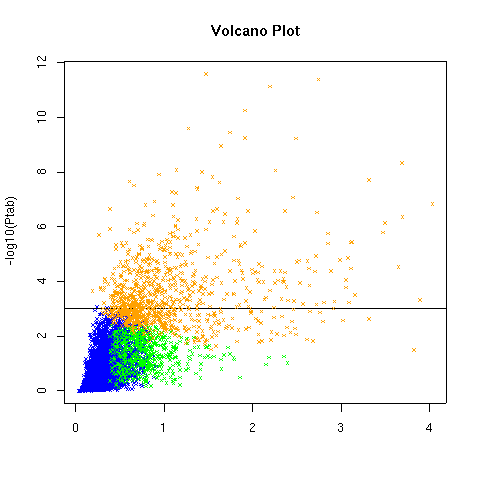
\includegraphics{volcano.png}
\caption{Volcano plot for kidney data - fixed effect model}
\label{fig:volcano}
\end{figure}
Note that the return variable of volcano contains the indices
for significant genes.

Now we can do cluster bootstrapping and build consensus trees.
Currently two cluster methods are implemented; K-mean and hierarchical clustering. Hierarchical cluster could be very sensitive to bootstrap
if you have too many leaves on the cluster. 
Some small disturbance on the data could change the whole tree structure. 
Suppose you have many genes, say, more than 50, and you want to build a
consensus tree from 100 bootstrapped hierarchical trees. Then it is very
likely that you will get a comb, that is, all leaves are directly under 
root. But if you only have a few genes to cluster, it is working fine. 
So we recommend to use K-means to cluster the genes and use hierarchical
to cluster the samples. 

\Rfunction{macluster} is the function to 
do cluster bootstrapping and \Rfunction{consensus}
is used to build consensus trees (groups for K-means) from the 
bootstrap results.
\begin{Sinput}
R> cluster.kmean <- macluster(fit.fix, ,term="Sample",
         idx.gene=idx.fix$idx.all,what="gene", method="kmean",
         kmean.ngroups=5, n.perm=100)
R> con.kmean <- consensus(cluster.kmean, 0.7)
\end{Sinput}
An expression profile plot will be generated for the consensus K-means
result. The plot is shown in Figure \ref{fig:vgprofile}.

\begin{figure}
\centering
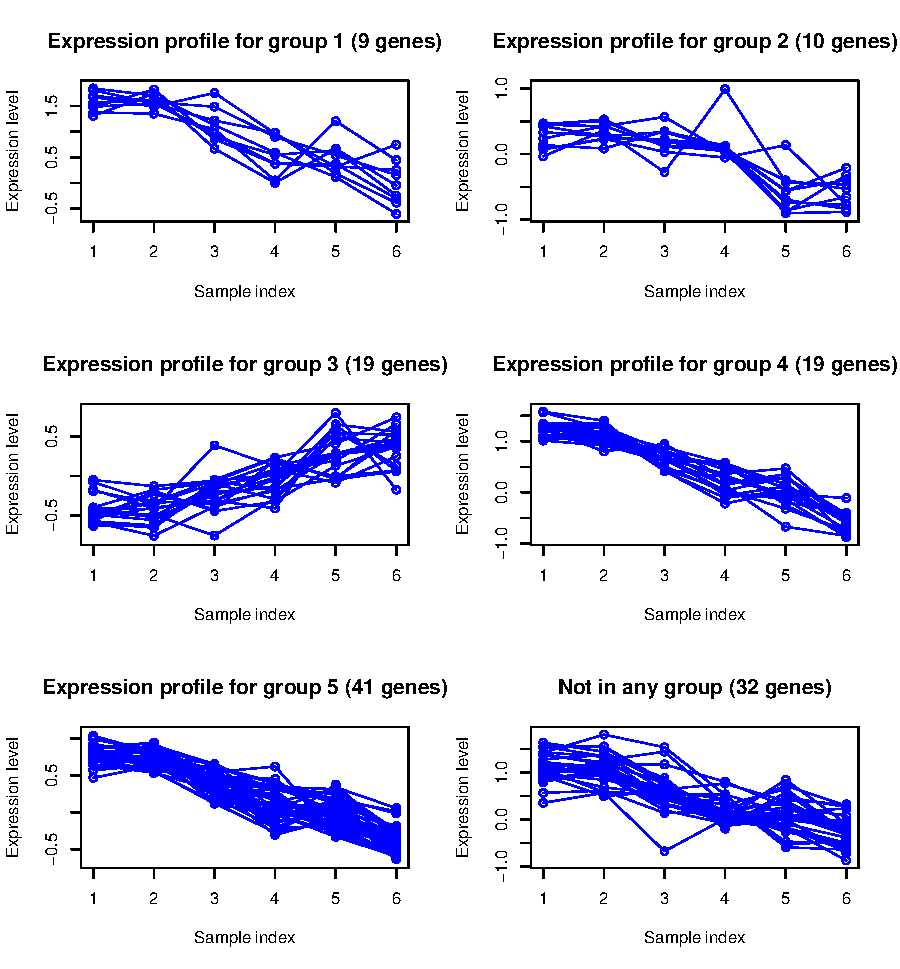
\includegraphics{vgprofile}
\caption{Expression profile plot for bootstrap K-means result, kidney data}
\label{fig:vgprofile}
\end{figure}

Now we can do hierarchical cluster on the samples. The consensus tree 
is shown in Figure \ref{fig:hckidney}.
\begin{Sinput}
R> cluster.hc <- macluster(fit.fix, term="Sample",
     idx.gene=idx.fix$idx.all,what="sample", method="hc", n.perm=100)
R> con.hc <- consensus(cluster.hc)
\end{Sinput}

\begin{figure}[htbp]
\centering
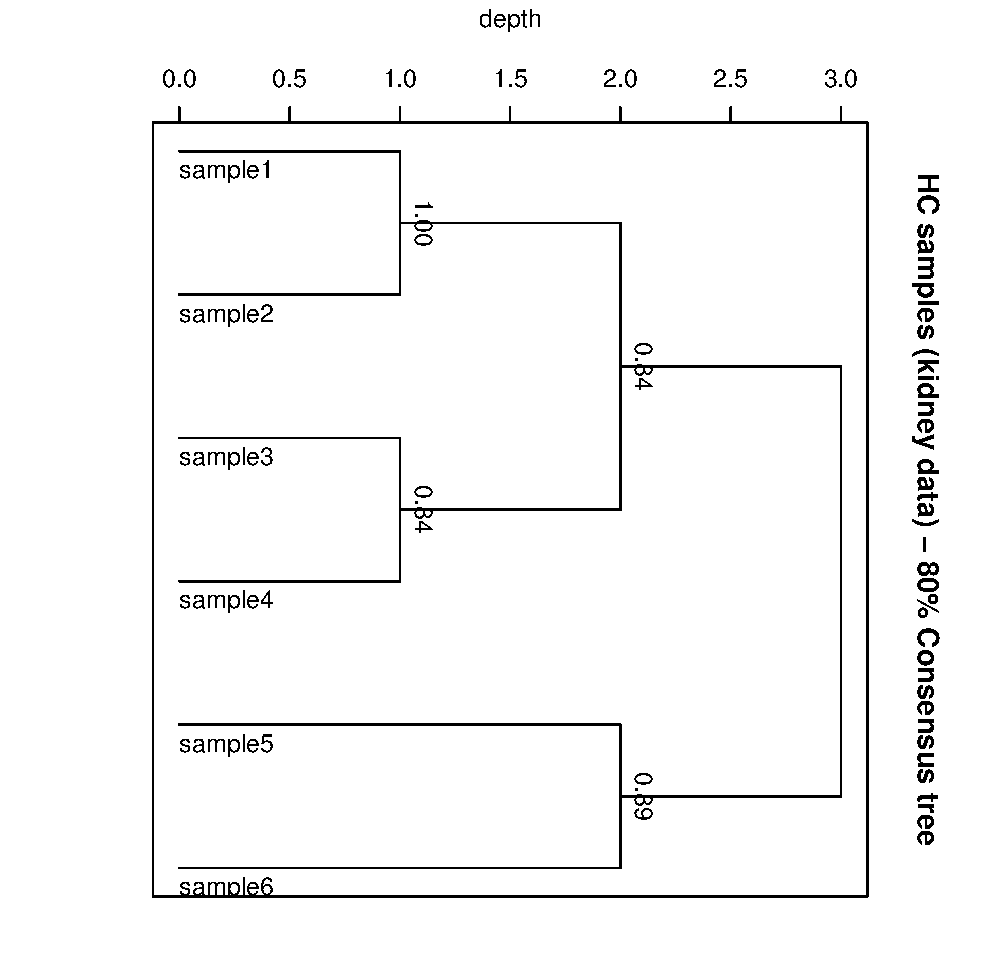
\includegraphics{hckidney}
\caption{80\% Consensus tree for bootstrapping hierarchical cluster on the samples,
kidney data}
\label{fig:hckidney}
\end{figure}
